\section{Motivating Example and Background}

We use a realistic example to discuss 
why existing techniques cannot satisfy the technical requirement well, why the technical problem is important, the basic idea of our strategy, and the insights behind our strategy.

Our example is from \blank{a realistic source}. It contains \blank{} components/steps. First, \blank{some basic introduction to the example}. Second, \blank{some basic introduction to the example}.Third, \blank{some basic introduction to the example}.

\subsection{Why Existing Techniques Cannot Satisfy Technical Requirement Well}
\explain{More details than the intro}
Existing techniques cannot satisfy the requirement because they fail to consider \blank{}. There are \blank{} types of existing techniques, but none of them can satisfy the requirement. \explain{Here is an example.} The first type is \blank{}, which cannot satisfy the requirement because \blank{}. For example, in Figure~\ref{fig:example}, \blank{the first type of technique cannot handle the code in lines 73-76. Therefore, it cannot do A that satisfy the requirement}. 

\begin{figure*}[t!]
    \centering
    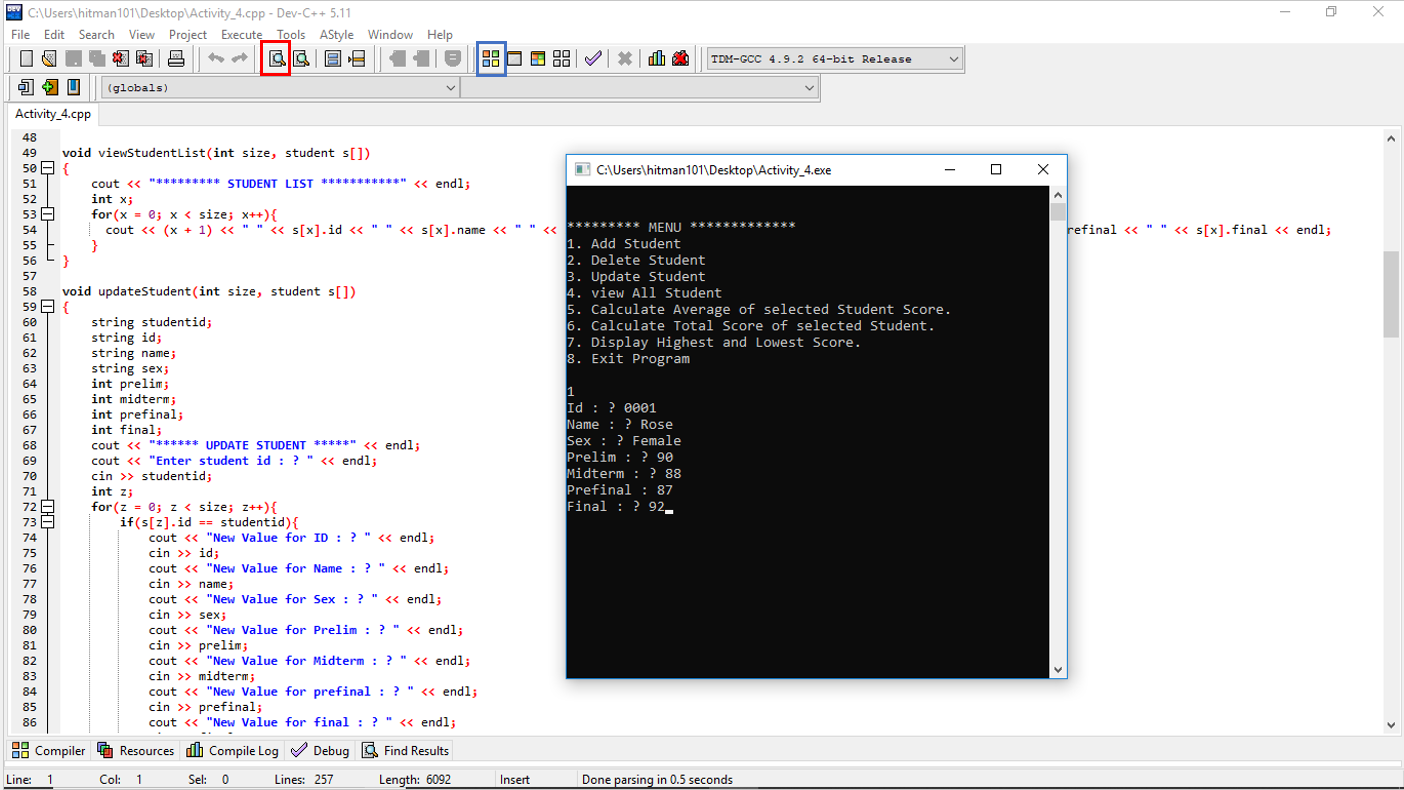
\includegraphics[width=\textwidth]{fig/example.png}
	\caption{Your beaultiful example picture}
	\label{fig:example}
\end{figure*}
\subsection{Why the Technical Problem Is Important}
The technical problem is important because \blank{}. Failing to address the problem well cause \blank{}. \explain{Here is an example.} For example, in Figure~\ref{fig:example}, the technical problem is critical to \blank{solve the constraints in the red box, so the requirement is not satisfied because of A}.

\subsection{Why the Technical Problem Is Challenging}
The technical problem \blank{} is challenging because of \blank{term 1}, \blank{term 2}, and \blank{term 3}. \explain{Here is an example.} \blank{Term 1} is challenging because \blank{}. For example, in Figure~\ref{fig:example}, \blank{term 1} introduces challenges in \blank{solving the constraints in the blue box}. Unfortunately, addressing \blank{term 1} is \blank{an NP-hard problem}. Existing techniques \blank{can only provide an approximate,}which is not sufficient to address the technical problem because \blank{}.   

\subsection{Our Insights}
Our strategy is based on \blank{} insights, which are \blank{},\blank{}, and \blank{}. \explain{Here is an example} For \blank{insight 1}, it is valid because \blank{}. For example, in Figure~\ref{fig:example}, \blank{the code in lines 81 - 88} they meet the \blank{insght 1} becuase \blank{}.  

\subsection{Core Idea}
The core idea of our strategy consists of \blank{} steps. \explain{Here is an example.} First, based on \blank{insight 1}, it does \blank{}. For example, in Figure~\ref{fig:example}, our strategy first \blank{identifies the code that meets requirement A, such as the code in lines 85-87}. This step is good because \blank{}. Second, based on \blank{insight 2}, it does \blank{}. For example, in Figure~\ref{fig:example}, our strategy does \blank{}. This step is good because \blank{}.

